\documentclass{article}
\usepackage{xcolor}
\usepackage{tikz}
\usepackage{pgfplots}
\usepackage{pgf-pie}

\definecolor{transfertoserver}{HTML}{D7191C}
\definecolor{database}{HTML}{FDAE61}
\definecolor{transfertoclient}{HTML}{ABDDA4}
\definecolor{rendering}{HTML}{2B83BA}


\begin{document}

\begin{figure}
\centering
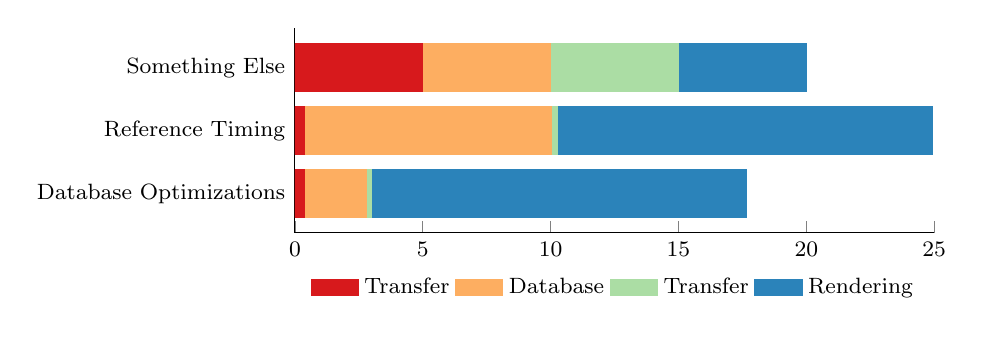
\begin{tikzpicture}
\begin{axis}[
    xbar stacked,
    legend style={
        legend columns=4,
        at={(xticklabel cs:0.5)},
        anchor=north,
        draw=none
    },
    ytick=data,
    axis y line*=none,
    axis x line*=bottom,
    tick label style={font=\footnotesize},
    legend style={font=\footnotesize},
    label style={font=\footnotesize},
    xtick={0,5,10,15,20,25},
    width=.8\textwidth,
    bar width=6mm,
    xlabel={Time in Seconds},
    yticklabels={Database Optimizations, Reference Timing, Something Else},
    xmin=0,
    xmax=25,
    area legend,
    y=8mm,
    enlarge y limits={abs=0.625},
]
\addplot[transfertoserver,fill=transfertoserver] coordinates
% Transfer
{(0.38,0) (0.38,1) (5,2)};
\addplot[database,fill=database] coordinates
% Database
{(2.4,0) (9.66,1)(5,2)};
\addplot[transfertoclient,fill=transfertoclient] coordinates
% Transfer
{(0.23,0) (0.23,1)(5,2)};
\addplot[rendering,fill=rendering] coordinates
% Rendering
{(14.66,0) (14.66,1)(5,2)};
\legend{Transfer,Database,Transfer,Rendering}
\end{axis}
\end{tikzpicture}
\caption{Performance Benefit by Database Optimizations}
\label{fig:performance:database}
\end{figure}

%%%%%%%%%%%%%%%%%%%%%%%%%%%%%%%%%%%%%%%%%%%%%%%%%%%%%%%%%%%%%%%%%%%%%%%%%%%%%%%%
%%%%%%%%%%%%%%%%%%%%%%%%%%%%%%%%%%%%%%%%%%%%%%%%%%%%%%%%%%%%%%%%%%%%%%%%%%%%%%%%
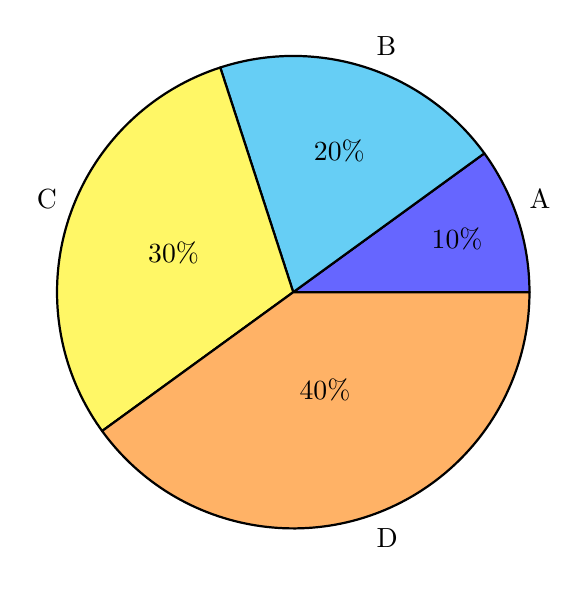
\begin{tikzpicture}
  \pie{10/A, 20/B, 30/C, 40/D}
\end{tikzpicture}
%%%%%%%%%%%%%%%%%%%%%%%%%%%%%%%%%%%%%%%%%%%%%%%%%%%%%%%%%%%%%%%%%%%%%%%%%%%%%%%%
%%%%%%%%%%%%%%%%%%%%%%%%%%%%%%%%%%%%%%%%%%%%%%%%%%%%%%%%%%%%%%%%%%%%%%%%%%%%%%%%
\end{document}
